\chapter{Anwendungsfall: Problembeschreibung}

In diesem Kapitel soll eine umfassende Beschreibung des Problems erfolgen,
aus welcher sich wiederum die Aufgabenstellung ergibt. Diese dann im
späteren Verlauf umgesetzt wird.

Den Anfang macht die Zielachitektur, welche primär aus Webtechnologien
besteht und somit zur Darstellung des Dokumentes dient. Siehe
Abschnitt \ref{sec-zielarchitektur}.

Die Zielarchitektur soll von einem Benutzer ohne großen Aufwand
generierbar sein und dabei die Möglichkeit haben, bestimmte
Aufgaben automatisch zu erledigen, wie z.B. das Zusammenstellen
eines Inhaltsverzeichnisses. Siehe Abschnitt \ref{sec-dsl}.

Damit aus der Schnittstelle die dem Benutzer gegebenen ist die Zielarchitektur
generiert werden kann, muss es eine geeignete Brücke bzw. Verbindung
geben, welche in Abschnitt \ref{sec-verbindung} näher beschrieben wird.

\section{Allgemeiner Aufbau von Dokumenten}

Vor allem akademische Dokumente wie z.B. Bücher, Patente oder Bachelorarbeiten
haben alle im Groben einen ähnlichen Aufbau. Daher ist es sinnvoll ersteinmal
allgemeine Ableitung über die Struktur solcher Dokumente zu machen, so dass
später daraus eine Architektur für nachfolgende Implementierungen enstehen kann.

Die wichtigsten Unterteilungen,
  wie auf Abbildung \ref{fig-areal_pages_entities} dargestellt,
werden hier grob definiert als

\begin{itemize}
  \item Dokumenten\emph{areal}.
        Beispielsweise gliedert sich diese Bachelorarbeit in die
        Areale Titelseiten, Inhaltsverzeichnis, Hauptdokument, Anhang und
        Literaturverzeichnis auf.
  \item Seiten.
        Jedes Dokument kann eventuell verschiedenartige Seiten haben, aber zumindest
        eine Standardseite, wie z.B. vertikales DIN A4, muss vorhanden sein.
        Aber auch innerhalb des Dokuments kann es verschiedenartige Seiten
        geben, wie z.B. horizontale Seiten für extra bereite Tabellen oder
        Titelblätter mit speziellem Layout.
  \item Entitäten.
        Das sind die einzelnen Einheiten wie Überschriften, Texte, Tabellen
        oder Bilder woraus sich schlussendlich das Dokument zusammensetzt.
\end{itemize}

\begin{figure}[h!]
  \centering
    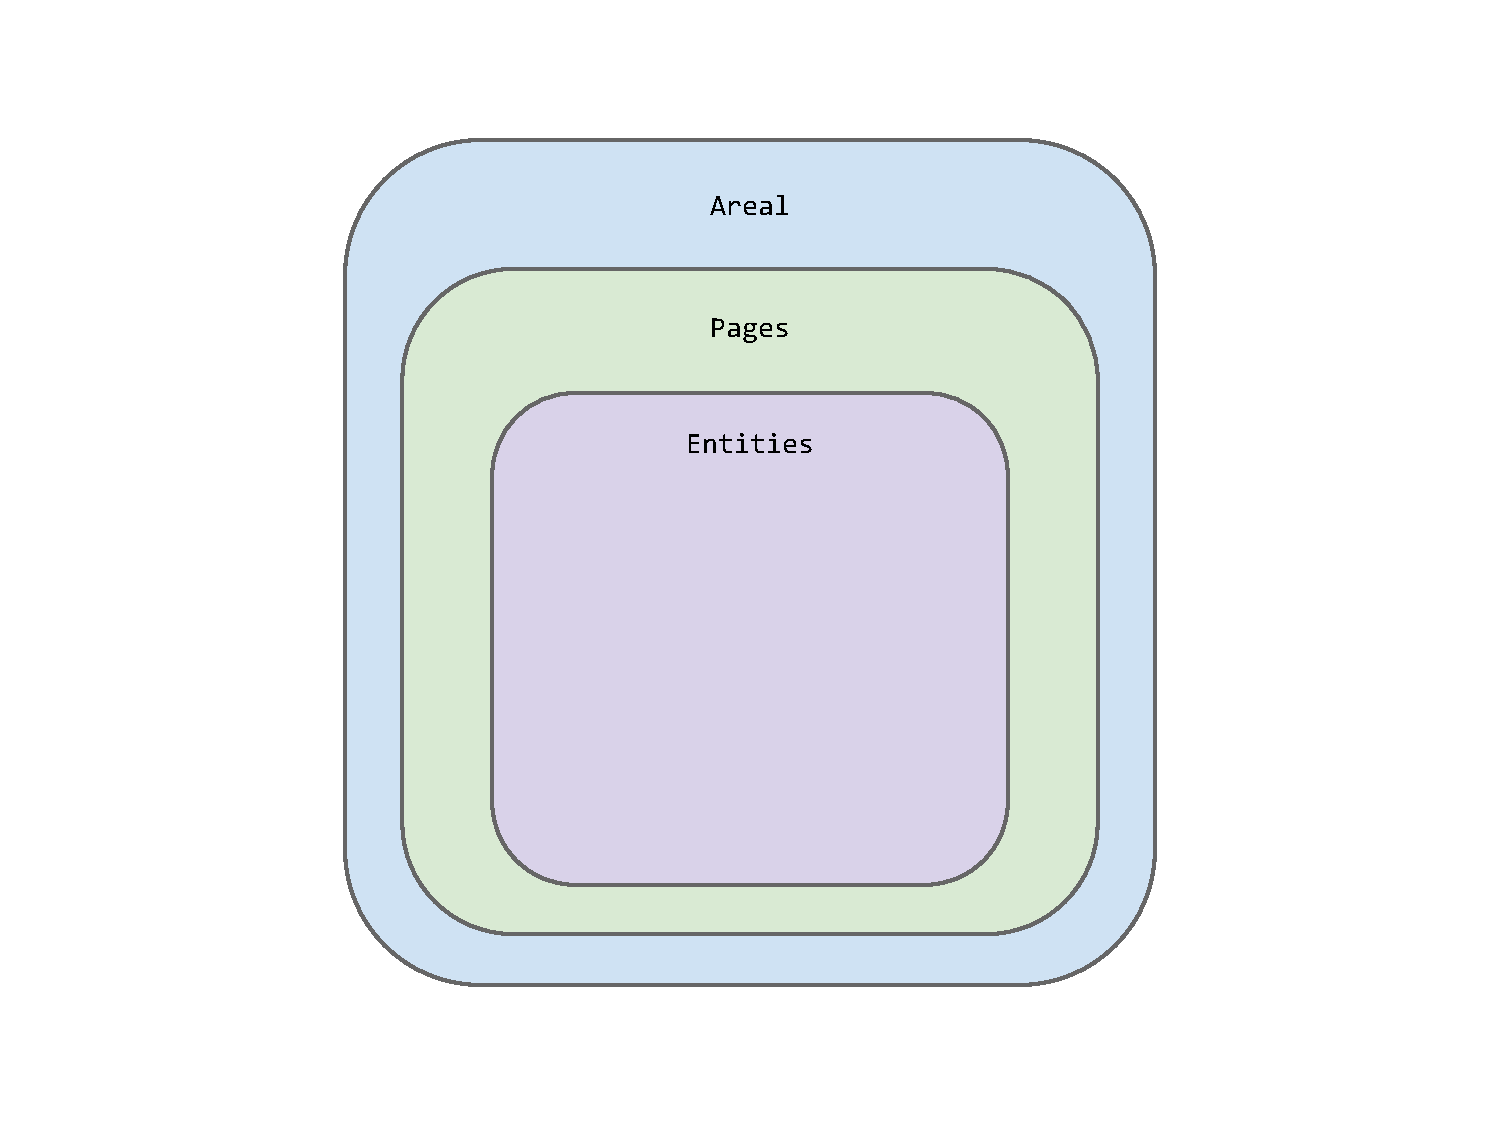
\includegraphics[width=0.9\textwidth]{figures/areal_pages_entities.pdf}
  \caption{Ein Dokument kann hierachisch grob in Areal, Seiten und Entitäten gegliedert werden.}\label{fig-areal_pages_entities}
\end{figure}

\section{Zielarchitektur}\label{sec-zielarchitektur}

Die primäre Aufgabe der Zielarchitektur ist es ein Dokument in
einem Webbrowser darzustellen. Das Dokument ist aber keine gewöhnliche
Webseite, sondern orientiert sich hautsächlich an akademischen
Dokumenten wie z.B. Fachbüchern. Bücher bestehen aus einzelnen Seiten,
welche in Webseiten in ihrer Ursprünglichen Form nicht vorgesehen sind.
Lange Dokumente werden mit Webtechnologie für gewöhnlich stufenlos
dargestellt, also alles auf einer einzelnen „Seite.“
Daher ist die Hauptaufgabe der Zielarchitektur eine \emph{Abstraktion
über Seiten} für Webtechnologie zu schaffen.

Die eigentliche Problematik ist hierbei, dass der Webbrowser fließenden
Text nicht selbst auf definierte Seiten umbrechen kann. Für den Browser
gibt es nur eine Seite, die quasi einem langen Textschlauch entspricht,
wenngleich er durch HTML struktuirert und
CSS-Eigenschaften gestaltet werden kann.

Damit verbunden ist die Problematik der
\emph{Zuordnung der einzelnen Dokumenten-Entitäten zu den Seiten},
dabei kann es dazu kommen dass eine Entität zwischen zwei Seiten
\emph{überlappt} und diese sollte, wenn möglich passend aufgeteilt werden.

Dadurch dass die Zielarchitektur sich um die Erstellung der Seiten und
die Zuteilung der Entitäten kümmern muss, ist es vollkommen natürlich,
dass sich diese auch der \emph{Durchnummerierung der Seiten} annehmen muss.
Davon hängt auch dirket die Funktion, die einzelnen Punkte des
Inhaltsverzeichnisses mit der entsprechden Seitennummer zu versehen, ab.

Zudem sollte es möglich sein, dass es \emph{verschiedene Arten von Seiten}
gibt, z.B. Deckblatt, normale vertikale Seite und horizontale Seiten für
große Tabellen oder Abbildungen. Oder auch dass verschiedene Papierformate
wie DIN-A4 oder US-Letter zur Auswahl stehen.

Die Einführung von \emph{Dokumenten-Arealen} als eine weitere hilfreiche
Abstraktion die zur Gliederung eines -- insbesondere
akademischen -- Dokuments dient, ist mit Sicherheit wünschenswert.
Damit soll es möglich sein, Dinge wie beispielsweise
Deckblatt, Inhaltsverzeichnis, eigentliches Dokument
und Literaturverzeichnis etc. von einander zu separieren, um für eine
flexiblere Konfiguration zu bieten. Beispielsweise um Areale in der Anordnung zu
verändern, oder Dinge wie Nummerierungen zu modifizieren, es wird z.B.
gerne der Anfang eines Dokuments mit römischen Ziffern durchnummeriert
und das eigentliche Dokument jedoch mit arabischen Ziffern.

% Seitennummerierung
% Inhaltsverzeichnis, Seite zuordnen
% Dokumentenareale
% Vorteile die sich durch die HTML-Nutzung ergeben? Welches Kapitel?

\paragraph{Aufgaben} auf einen Blick zusammengefasst:

\begin{itemize}
  \item Abstraktion für Seiten,
  \item Zuordnung der Entitäten auf Seiten,
  \item Behandlung überlappender Entitäten,
  \item Ermöglichung verschiedener Seiten-Arten,
  \item Durchnummerierung der Seiten,
  \item Seitenzugehörigkeit von Entitäten bestimmbar,
  \item Dokumenten-Areale zur Strukturierung.
\end{itemize}


\section{Domain-Specific Language}\label{sec-dsl}

Die \emph{domain-specific language}, kurz \emph{DSL}, stellt die
textuelle Schnittstelle zwischen Benutzer und der Zielplatform dar.
Eine DSL ist eine leichtgewichtige Programmiersprache, die für den
Einsatz ihres Spezialgebietes, ihrer Domäne bzw. ihres Aktionsraumes,
zugeschnitten ist.

Dabei unterscheidet man grob zwischen \emph{internen}, \emph{externen}
und \emph{nicht-textuellen} DSLs.\cite{dsls} Da in diesem Projekt allerdings
nur eine textuelle DSL zum Einsatz kommen soll, konzentrieren wir uns
auf die internen DSLs bzw. externen DSLs.

\paragraph{Definition interne DSL}
\begin{quote}
Eine interne DSL wird als Bibliothek auf Basis
einer bereits existierenden Wirtssprache implementiert. Das interne DSL-Skript
ist eine dünne Fassade über die Abstraktionen der unterliegenden Wirtssprache.
\end{quote} (von \cite{dsls} Kapitel 1.5.1, Seite 18.)

\paragraph{Definition externe DSL}
\begin{quote}
Eine externe DSL wird von Grund auf entwickelt und hat eine separate
Infrastruktur für die lexikalische Analyse, Interpretation, Kompilierung
und Code Generierung. Eine externe DSL zu entwickeln ist gleichzusetzen mit
der Implementierung einer neuen Sprache von Grund auf, welche ihre eigene
Syntax und Semantik hat.
In den meisten Fällen findet man externe DSLs vor, welche nicht alle
Komplexitäten einer vollwertigen Sprache benötigt.
\end{quote} (von \cite{dsls} Kapitel 1.5.2, Seite 18f.)

\paragraph{Ausgewählt und gegenübergestellt werden}

\begin{itemize}
  \item die Scala-Programmiersprache für interne DSLs,
  \item das Xtext-Framework für externe DSLs.
\end{itemize}

Warum genau diese zwei Vertreter sich besonders eigenen und ausgewählt wurden,
wird in Kapitel \ref{sec-warumAusgewaehlt} beschrieben.

\subsection{\TeX, eine DSL für Dokumente}

\TeX~ ist eine weit verbreitete Programmiersprache die speziell für die
Aufgaben eines Textsatzsystem erschaffen wurde. Daher kann man
\TeX~ auch als eine \emph{externe DSL} ansehen.
In diesem Abschnitt wird etwas auf
\TeX~ eingegangen, da insbesondere diese Programmiersprache als Inspiration
bzw. Vorbild dient.


\subsubsection{Herkunft und Grundlagen}

Der Name hat seinen Ursprung aus dem griechischen $\tau\epsilon\chi$,
welches auch die Wurzel für das englische Wort \emph{technology} ist.
$\tau\epsilon\chi$ bedeutet also Technologie, aber auch Kunst.
(\cite{tex-a}, Kapitel 1, Seite 1)

\TeX~ ist ein Dokumenten-Compiler, welcher dazu gedacht ist hochqualitativen
Textsatz zu erstellen, mit einem starken Fokus auf
Mathematik. \TeX82 ist in der Programmiersprache Pascal-H definiert
bzw. in WEB. (\cite{tex-b}, §1, Seite 1)

Die prototypische Entwicklung begann im Sommer 1977, Version 0 wurde
im September 1982 fertig gestellt, seit dem wurde TeX eingefroren
und seither wird nur noch an der Stabilität und Zuverlässigkeit
gearbeitet. (\cite{tex-b}, §2, Seite 2)

Es gibt etwa 300 \TeX~Kontrollsequenzen, sog. „Primitive“ welche das
Low-Level TeX bilden. Diese Primitiven sind atomisch und werden nicht weiter
in kleinere Funktionen zerlegt.
Zudem kommen noch etwa 600 weitere, aus Primitiven zusammengesetzte,
Kontrollsequenzen „plain \TeX“ dazu,
die zusammen mit den Primitiven das Standard-\TeX~bilden.
(\cite{tex-a}, Kapitel 3, Seite 9--11)

\TeX~ hat eine \emph{REPL}\footnote{REPL steht für read–eval–print loop,
eine interaktive Programmierumgebung. Scala besitzt auch eine REPL.
Dieser kann unter UNIX mit dem Befehl \lstinline|tex| aufgerufen werden.}
in welcher interaktive Programmiersitzungen abgehalten werden können,
wie z.B.:

\paragraph{Primitiv}

\begin{verbatim}
**\show\input
> \input=\input.
\end{verbatim}

\paragraph{Zusammengesetzte Kontrollsequenz, ein Makro}

\begin{verbatim}
**\show\TeX
> \TeX=macro:
->T\kern -.1667em\lower .5ex\hbox {E}\kern -.125emX.
\end{verbatim}

Viele Ligaturen\footnote{Ligaturen wie z.B. \lstinline|ff| zu ff}
werden von TeX als solche erkannt und direkt also solche
im resultierenden Dokument umgesetzt. Zudem können mit einer gewöhnlichen
Tastatur auch ungewöhnliche Zeichen gesetzt werden, so kann z.B. mit der
\lstinline|\ss| \TeX-Sequenz ein ß gesetzt werden, was dem Dokument
schöne Typographie bzw. Zeichen anderer Sprachen, mit lateinischen
Zeichen, erlaubt. (\cite{tex-a}, Kapitel 9, Seite 51--52)

Jedes einzelne Zeichen ist eine Box welche, aus Höhe, Breite, Tiefe und
einer Basisline besteht, diese Boxen können
zu größeren Einheiten „verklebt“ werden, so dass daraus schlussendlich
auch komplizierte Seiten-Layouts zusammengestellt werden können.
(\cite{tex-a}, Kapitel 11, Seite 63)

\begin{figure}[h!]
  \centering
    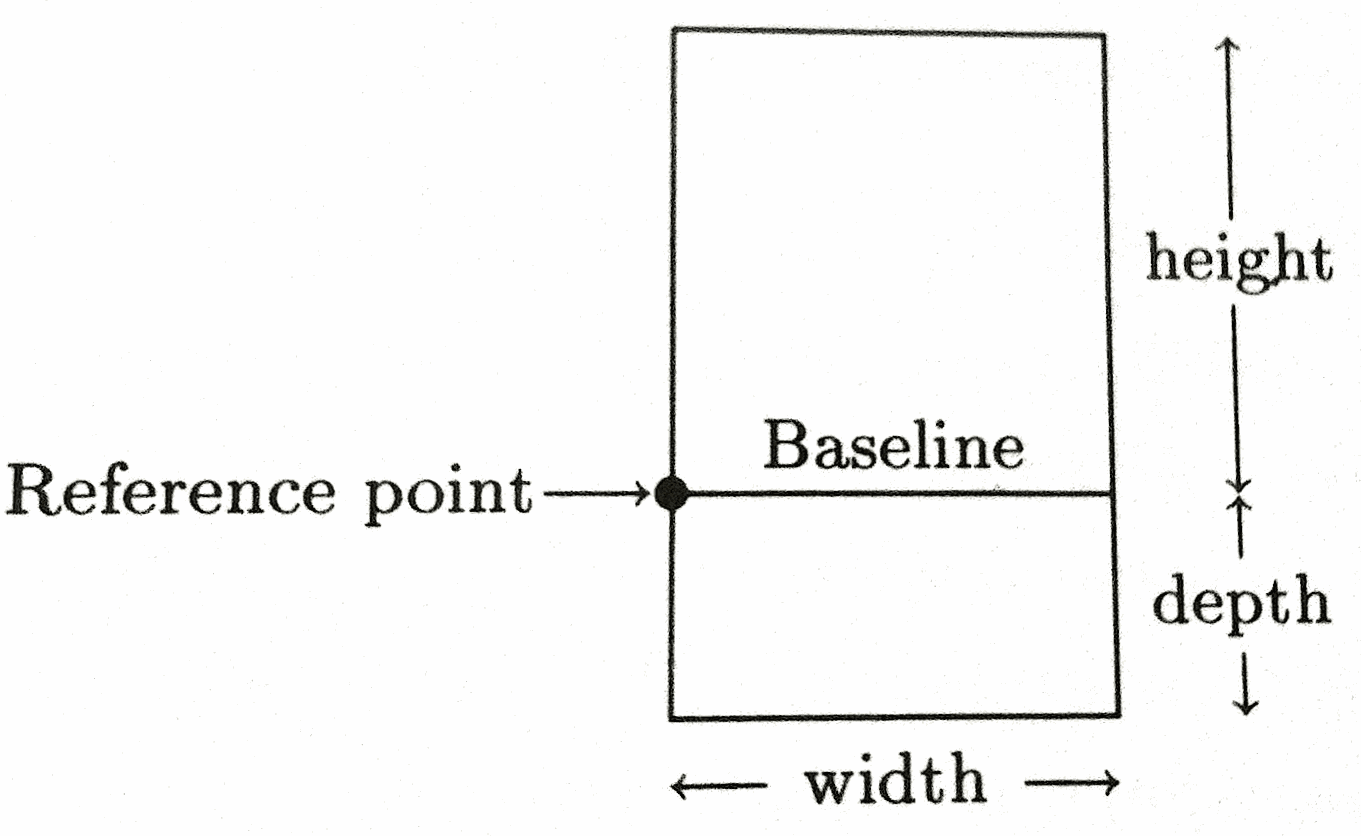
\includegraphics[width=0.5\textwidth]{figures/tex_box.png}
  \caption{\TeX~ Box für jedes einzelnes Zeichen.
           (\cite{tex-a}, Kapitel 11, Seite 63)}\label{fig-tex_box}
\end{figure}

\TeX~ kann einen Abschnitt in einzelne Zeilen herunterbrechen, so dass
der Benutzer sich nicht um diese Aufgabe kümmern muss. Es wird der beste
Weg gesucht, für den jeweiligen Abschnitt das „minimale Übel“ zu finden.
(\cite{tex-a}, Kapitel 14, Seite 91)
Die Methode die in TeX verwendet wird, geht auf Michael F. Plass
und Donald E. Knuth zurück. (\cite{tex-b}, §813, Seite 343)
Zudem ist ein Silbentrennungsalgorithmus enthalten, der auf
Frank M. Liang zurückgeht. (\cite{tex-b}, §919, Seite 386)

Das Dokument in einzelne Seiten zu unterteilen kann \TeX~ automatisch
vornehmen. Machmal ist es allerdings geschickter, wenn der Dokumentenersteller
mit etwas Handarbeit den Seitenumbruch selbst einstellt, um ein ideales
Ergebnis zu erzielen. (\cite{tex-a}, Kapitel 15, Seite 109)

\subsubsection{Fähigkeiten als Programmiersprache}

Mit den geschweiften Klammern \{ und \} sind die Gruppierungssymbole, so
dass Änderungen innerhalb einer Gruppe nicht auch Dinge außerhalb
verändern. (\cite{tex-a}, Kapitel 5, Seite 19)
Das Verhalten ist also gewohnt wie es in Programmiersprachen wie C,
Java oder Scala vorkommt.

Makros bzw. Definitionen ermöglichen es Abkürzungen für z.B. häufig
verwendete Kontrollsequenzen anzulegen, so dass insbesondere
der Quellcode übersichtlicher wird bzw. der Dokumentenersteller sich
Schreibarbeit sparen kann.

\begin{verbatim}
\def\xvec{(x_1,\ldodts,x_n)} --> \xvec
\end{verbatim}

TeX expandiert dann automatisch das Makro für den Benutzer.
So ist es sinnvoll wenn TeX-Benutzer ihre eigene kleine Bibliothek mit
Makros zusammenstellen, so dass sie diese in verschiedenen Dokumenten
wiederverwenden können. (\cite{tex-a}, Kapitel 20, Seite 199)
\LaTeX~ ist \emph{u.a.} eine sehr bekannte und beliebte
Bibliothekszusammenstellung\footnote{\url{http://www.latex-project.org}}.

\begin{verbatim}
\input macros  % Importiert aus macros.tex
\end{verbatim}

Parametrisierte Makros sind auch möglich, was TeX eine mächtige
Makroprogrammierfähigkeit verschafft:

\begin{verbatim}
\def\cs #1. #2\par{...}
\end{verbatim}

Wobei in diesem Beispiel nach Aufruf von \lstinline|\cs| Parameter
\lstinline|#1| so lange gilt,
bis \lstinline|". "| auftritt und Parameter \lstinline|#2|
bis \lstinline|'\par'| auftritt. (\cite{tex-a}, Kapitel 20, Seite 202)

Die Makros können auch rekursiv aufgebaut werden, so dass damit auch möglich ist
Schleifen (tail recursive) zu bilden.
(\cite{tex-a}, Kapitel 20, Seite 219)
TeX selbst bietet auch ein \lstinline|\loop...\repeat| Kommando an,
mit dessen Hilfe Schleifen gebildet werden können.
(\cite{tex-a}, Kapitel 20, Seite 217)


\paragraph{Einer Kontrollsequenz eine Bedeutung zuweisen:}

\begin{itemize}
  \item \lstinline|\font\cs=<font name>|
        (\lstinline|\cs| wird ein font identifier),
  \item \lstinline|\chardef\cs=<number>|
        (\lstinline|\cs| wird ein character code),
  \item \lstinline|\countdef\cs=<number>|
        (\lstinline|\cs| wird ein \lstinline|\count| register,
        was quasi einer int Variablen entspricht),
  \item \lstinline|\def\cs...{...}|
        (\lstinline|\cs| wird ein Macro),
  \item \lstinline|\let\cs=<token>|
        (\lstinline|\cs| bekommt die Bedeutung des Tonkens)
\end{itemize}

\paragraph{Beispiel}

\begin{verbatim}
\let\a=\macroname
\end{verbatim}

\lstinline|\a| wird zu \lstinline|\macroname| aufgelöst, quasi wie eine Referenz.
(\cite{tex-a}, Kapitel 20, Seite 206)


Makros können auch ihr Verhalten abhängig durch bestimmte Bedingungen
ändern, indem mit \lstinline|\if<condition><true text>\else<false text>\fi|
Bedingungen
aufgestellt werden. Es gibt verschiedene in TeX hart Codierte
\lstinline|<condition>|
wie z.B. \lstinline|\ifnum| zum Testen auf \lstinline|>, <, 0| eines count-Registers.
(\cite{tex-a}, Kapitel 20, Seite 207)
\TeX ~hat verschiedene if-Anweisungen wie \lstinline|\if|, \lstinline|\iftrue| oder \lstinline|\ifvoid| etc.,
diese Anweisungen sind fester Bestandteil der sprachlichen Grammatik.
(\cite{tex-a}, §487, Seite 197, §489, Seite 198)

\TeX~ unterstützt also Funktionsaufrufe in Form von Makros,
Verzweigungsentscheidungen
und rekursive Aufrufe bzw. Schleifen. Somit ist \TeX~ \emph{turing-vollständig.}

Auch hat TeX rudimentäre Eingabe/Ausgabe Fähigkeiten, indem es
bis zu 16 Dateien gleichzeitig öffnen und lesen kann, jedoch sind auch
diese Makros hart einkodiert wie z.B. \lstinline|\openin0=<filename>|.
Auch ist es möglich mit \lstinline|\message{...}| auf das Standard-Out zu schreiben
bzw. mit \lstinline|\read...to\varname| vom Standard-In zu lesen.
(\cite{tex-a}, Kapitel 20, Seite 217)

\subsubsection{Warum \TeX~ so aussieht, wie es aussieht}

Das Sprachdesign von \TeX~ ist auf Dokumentengenerierung ausgelegt, dies
bedingt, dass Zeichen bzw. Zeichenketten der Hauptbestandteil des Codes
sind. Der Benutzer will also so wenig wie möglich explizite Angaben über
Zeichenketten-Literale machen, daher fängt \emph{jeder Befehl} in \TeX~
mit einem \lstinline|\| an, zwar sehen die Befehle dann etwas gewöhnungsbedürftig
aus, aber daher kann alles andere als Zeichenkette vom Parser
wahrgenommen werden.

\TeX~ unterscheidet zwischen 16 Zeichenkategorien, um die Sprache zu parsen:

\begin{enumerate}
  \item Escape \lstinline|\|
  \item Gruppenbeginn \lstinline|{|
  \item Gruppenende \lstinline|}|
  \item Mahtemodus \$
  \item Alignment tab \lstinline|&|
  \item End of line \lstinline|<return>|
  \item Parameter \lstinline|#|
  \item Superscript \lstinline|^|
  \item Subscript \lstinline|_|
  \item Ignored character \lstinline|<null>|
  \item Space
  \item Letter \lstinline|A,...,z a,...,z|
  \item Other character (Keiner der anderen)
  \item Active character \lstinline|~|
  \item Kommentar \%
  \item Invalid \lstinline|<delete>|
\end{enumerate}

(\cite{tex-a}, Kapitel 7, Seite 37)

\subsubsection{Was \TeX~ generiert}

Hier ein kleines Basisskript, welches so in den REPL getippt werden kann und
eine gesetzte \lstinline|textput.dvi| Datei produziert:

\begin{verbatim}
**\relax
*Hello World!
*This is \TeX
*\end
\end{verbatim}

TeX verwendet internen immer den eigenen Zeichencode und konvertiert beispielsweise
\lstinline|'b'| immer in die \TeX-Sequenz \lstinline|\char98| um.
(\cite{tex-a}, Kapitel 8, Seite 43)

Das \emph{device-independent file format (DVI)} ist ein Stream aus
8-Bit bytes, welche eine Serie an
Maschinencode ähnliches Kommandos enthält, zur Zeichnung eines Dokuments.
\TeX~ liefert die Seiten in Form einer DVI-Datei aus.
(\cite{tex-b}, §583, Seite 234, §584, Seite 235, §592, Seite 244)

Die \TeX-Kontrollsequenzen sind auf Pascal Prozeduren abgebildet,
welche schlussendlich DVI-Dateien produzieren. Das bedeutet, dass der Generator
relativ fest verdrahtet und somit schwierig zu ändern ist.

\paragraph{Produktionsformat versus Auslieferungsformat}

\TeX~ stellt ein Konzept besonders klar dar: die \emph{Unterscheidung
zwischen Produktionsformat und Auslieferungsformat.} Diese Unterscheidung
wird von vielen Menschen nicht verstanden oder wahrgenommen; daher kommt
es immer mal wieder vor, dass Microsoft Word Dateien im E-Mail Anhang zu
finden sind.

Bei \TeX~ ist das Produktionsformat die Quellcode-Dateien und in neuerer
Zeit ist das Auslieferungsformat eine gesetzte PDF-Datei, welche auf jeder
Plattform gleich angezeigt wird und auch als Archivierungsformat tauglich
ist.


\subsection{Das DSL Idealbild}

Wie schon erwähnt, dient die DSL als Schnittstelle für den Benutzer,
und sollte möglicht leicht für diesen zu verstehen sein, so dass
auch ein Benutzer ohne große Programmierkenntnisse zumindest die
DSL verstehen und schreiben kann. Dies erfordert intuitive Konzepte,
klare Strukturen und übersichtliche bzw. leichtgewichtige Syntax, welche
sich auf das Domänen-Problem einer Dokumentengenerierung konzentriert.

In dem aufgeführten Pseudo-Code, ist aufgezeigt, wie die DSL im Idealfall
aussehen könnte, auch wenn diese von der realen Implementierung abweicht.
% TODO Referenz darauf, was daraus geworden ist!
% TODO Begründung, warum diese Abweichungen nötig sind -> und warum TeX so aussieht.

\begin{lstlisting}[language=DSL_ideal]
Use Template
    AcademicReport

Section
    Ueberschrift

Text
    Lorem ipsum dolor sit amet, consetetur sadipscing elitr,
    sed diam nonumy eirmod tempor invidunt ut labore et dolore
    magna aliquyam erat, sed diam voluptua. At vero eos et accusam et

Subsection
    Unterueberschrift

Text
    Lorem ipsum dolor sit amet, consetetur sadipscing elitr,
    sed diam nonumy eirmod tempor invidunt ut labore et dolore
    magna aliquyam erat, sed diam voluptua. At vero eos et accusam et

    Auf Abb. picName.figureNumber kann man erkennen ...

PythonScript named pyScriptName
    from matplotlib import pyplot
    from scaltex import return_to_document
    pyplot.plot(range(10))
    pic = pyplot.savefig("pic.png")  // Achtung Vereinfachung!
    return_to_document(pic)

Figure named picName
    src = pyScriptName  // oder z.B. auch moeglich "/home/pic.png"
    descr = Beschreibung des Bildes
\end{lstlisting}


\section{Verbindung zwischen DSL und Ziel}\label{sec-verbindung}

Aus den Eingaben die der Benutzer über die DSL-Schnittstelle gemacht hat,
muss nun das Ziel, Webtechnologie zur Darstellung im
Webbrowser, \emph{generiert} werden.

Dadurch, dass es viele \emph{verschiedene Dokumenten-Templates} geben kann,
z.B. eines für akademische Berichte und ein anderes für Patente, entsteht das
Problem dass zwar immer auf das gleiche Ziel (Webtechnologie) abgebildet
wird, aber dieses unterschiedliche Ausprägungen besitzen kann.
Jede dieser Ausprägungen kann sich in ihren Eigenschaften, Einsatzzielen
und Darstellungsmöglichkeiten (z.B. mathematische Formeln in einen
Dokument-Typ und chemische Formeln im Anderen) unterscheiden.

Ideal ist es wenn insbesondere die Darstellungsmöglichkeiten zwischen
den einzelnen Dokument-Typen \emph{austauschbar} sind, z.B. gefällt mir
die Tabelle aus dem \verb|Patent|-Template, aber ich möchte diese gerne im
\verb|Bericht|-Template verwenden.

Außerdem ist
es wünschenswert, wenn zwischen verschiedenen Dokumenten-Typen gewechselt
bzw. \emph{migriert} werden kann, ohne große Veränderungen am
DSL-Code vornehmen zu müssen, z.B. wird im
DSL-Skript nur die Programmzeile \verb|Bericht| durch \verb|Patent| geändert und
das Dokument bekommt ein völlig anderes Erscheinungsbild---die eines Patents.
Wobei natürlich diese beiden Ausprägungen Spezialisierungen des Typs
\verb|AkedemischesDokument| sein müssen, damit die Migration funktionieren kann.

